\chapter{INTRODUCTION}
Evolution has been intensively studied since the publication of \emph{On the Origin of Species} in order to untie the mysteries behind fascinating machineries within living systems. In a broader sense, most of the studies on evolutionary biology have two main goals: (I) To document history of life through evolutionary point of view, and (2) to understand causal mechanisms responsible for the biological diversity that we have on Earth \cite{futuyma2001evolution, hird2017evolutionary}. In addition to these goals, the idea of using pre-existing living systems as cell factories for industrial purposes gained close attention in the last decades \cite{nielsen2016engineering}.

Evolutionary engineering studies, adaptive laboratory evolution in particular, refers to the experiments in which the environmental conditions are altered gradually to obtain adapted populations in the laboratories \cite{garland2009experimental}. Accumulation of mutations obtained due to environmental alterations through generations, where the favored individuals (mainly the ones with increased fitness) are selected to become parents of the next generation, result a population with advantageous traits compared to starting population. Since one of the main challenges in the evolutionary engineering field is being able to analyze experimental to answer fundamental questions, adaptive evolution studies usually require interdisciplinary research in order to answer fundamental questions. What has changed in the cells through generations? What is the genetic basis for adaptation? Can we evolve any organism to any condition? If so, how? These questions and many more are asked every day, and the corresponding answers potentially give rise to more questions.

The purpose of this thesis is to enlighten metabolic changes in the adaptation of the yeast \emph{S. cerevisiae} using computational methods, specifically genome-scale metabolic models. Evolved yeast strains (such as ethanol tolerant, long-lived, multi-stress resistant strains) are going to be analyzed comparatively to the unevolved strains using intracellular flux distributions obtained with the integration of transcriptomics data. This study will also contribute to the global understanding of metabolic regulations in yeast, and will be further expandable into metabolic engineering studies.

\chapter{THEORETICAL BACKGROUND}

\section{Adaptive Laboratory Evolution}
Since the very first laboratory evolution experiment was published in the late 19th century by William Dallinger, technological advancements allowed researchers to employ fully-controlled experiments for strain engineering to achieve desired traits \cite{dragosits2013adaptive}. Challenges in the experimental design of evolutionary studies, such as maintenance of the generations, controlling the environment, and feasibility to perform data analysis make the use of microorganisms in evolutionary studies more suited, especially \emph{Escherichia coli} and \emph{Saccharomyces cerevisiae} given their extensive characterization \cite{mcdonald2019microbial}.

Commonly used approaches of adaptive laboratory evolution (ALE) include chemostat cultures and serial batch or colony transfers (Figure \ref{fig:ale}). Serial transfer experiments in which the initial population is aliquoted and transferred into a new medium are simpler and cheaper to set up, however the possibility of genetic drift is higher due to random sampling of the population. On the other hand, continuous systems such as chemostat experiments in bioreactors have advantages on maintaining constant growth rates and population sizes, but with increasing experimental cost \cite{winkler2013adaptive}.

\begin{figure}[ht]
\begin{center}
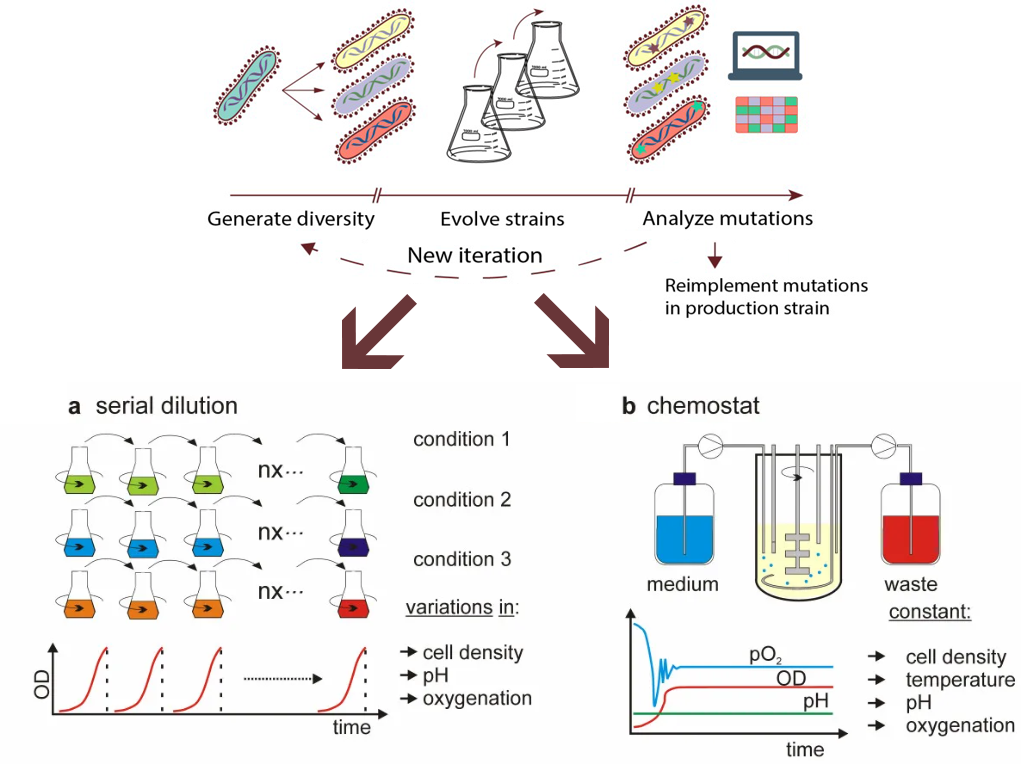
\includegraphics[width=1\columnwidth]{ALE.png}
\end{center}
\caption[Adaptive laboratory evolution workflow]{ALE methods and workflow. Figure is taken from \cite{dragosits2013adaptive} and \cite{shepelin2018selecting} and will be redrawn altogether.}
\vskip\baselineskip % Leave a vertical skip below the figure
\label{fig:ale}
\end{figure}

In addition to the methodological choice, decision of the selection criteria and the time span for the experiments are critical factors in ALE \cite{dragosits2013adaptive}. Growth rates, survivability in stressful environmental conditions and biomass yields are the most common fitness criteria for a population to be selected. Throughout the selection process, reaching \textgreater 500 generations may take a few weeks or a few months depending on the organism, therefore, detailed planning is essential \cite{conrad2011microbial}.

Capturing genomic changes in the dynamic evolution process is the main goal of an ALE study, therefore frequent data collection in longitudinal manner is a must to unveil molecular details. Next-generation technologies empower researchers to catch even single-nucleotide mutations through genome sequencing and also provide an understanding on broader regulatory changes through equation expression profiles \cite{conrad2011microbial}. Focus of the studying the differences between evolved and unevolved strains may be on the individual protein level or as a system-level trait. Interpreting the system as a network enables various ways to investigate causality behind adaptive mechanisms and dynamics of evolution \cite{soyer2013evolutionary, long2018adaptive}.

\subsection{Computational Tools for ALE Experiments}

Adaptive laboratory evolution, in laboratories, uses natural selection to capture microbial adaptations for decades. Although the results of these experiments would provide the ideal selection pressure to be imposed on organisms to obtain favored strains, the difference between the starting and the evolved strain is not easy to find. Throughout the years, various additional methods and computational tools are invested to investigate findings. With decreasing cost of whole genome sequencing and resequencing, identification of mutations can reveal the mystery behind the adaptations. Due to complexity of cellular systems and missing points in the metabolic regulations, the interpretation of the mutation effects is still the main challenge in the field \cite{palsson2011adaptive}.

A web-based database platform, ALEdb (aledb.org) \cite{phaneuf2019aledb}, has been created last year. Platform collects and reports on ALE acquired mutations and their experimental conditions and provides several feature such as searching for specific mutations within reports, exporting of mutation query results for custom analysis, and many more. With these useful features and being freely available for non-commercial uses, ALEdb becomes a resourceful tool in the field (Figure \ref{fig:intro_aledb}).
\vspace{1cm}
\begin{figure}[H]
\begin{center}
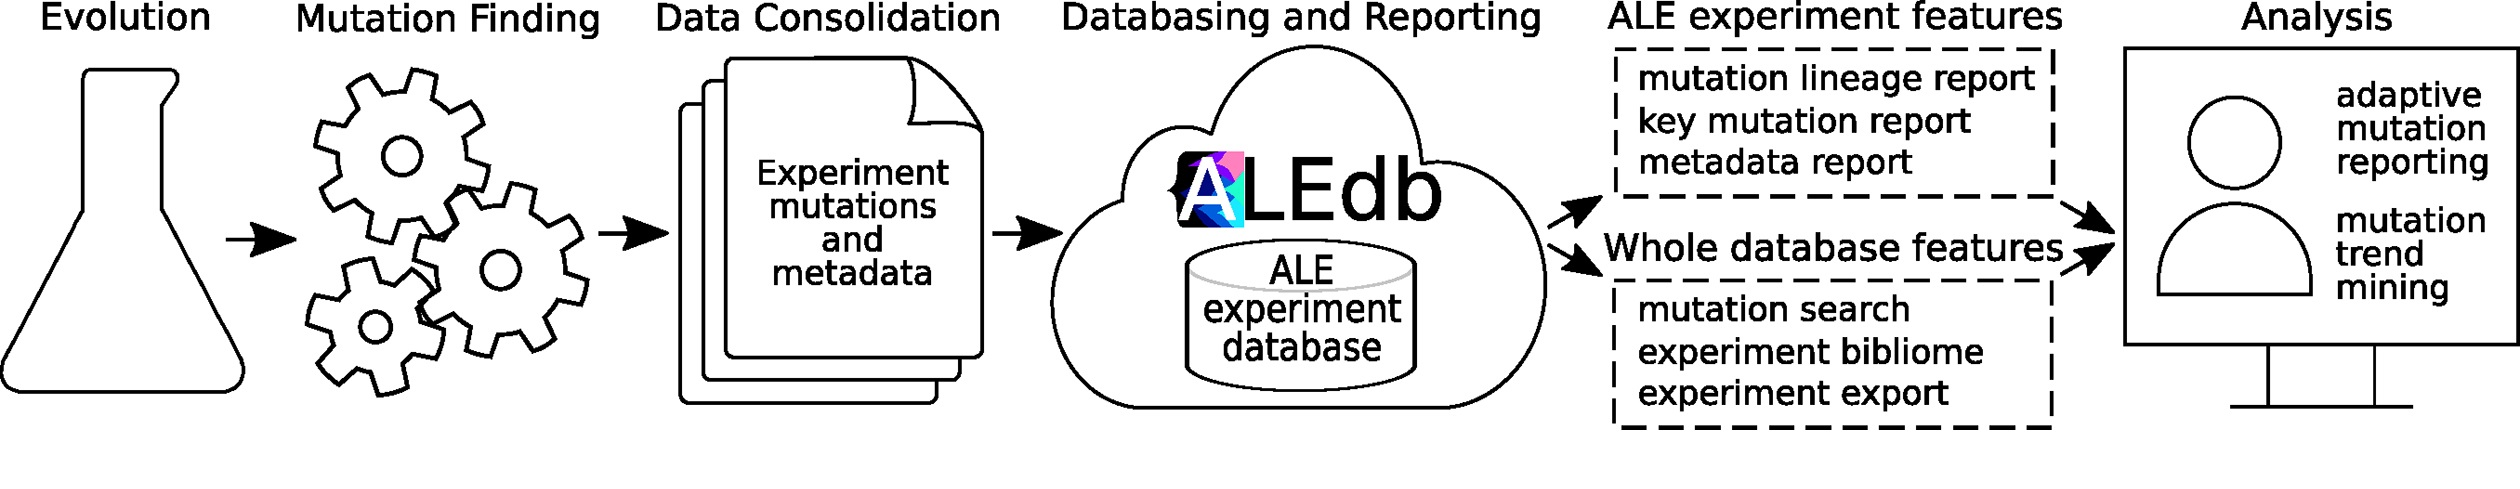
\includegraphics[width=1\columnwidth]{figures/intro_aledb.jpeg}
\caption[Illustrated pipeline of ALEdb from experimental design to reportingt]{Illustrated pipeline of ALEdb\cite{phaneuf2019aledb} from experimental design to reporting.}
\label{fig:intro_aledb}
\end{center}
\end{figure}

eVOLVER\cite{wong2018precise}, an open-source DIY framework that promises a solution to the main challenge of balancing the tradeoff between controllable (such as bioreactor designs) and throughput (such as batch designs) experiments in the ALE. Framework comes with both software and hardware, and it offers to define the various experimental parameters e.g. temperature, density, media, in a virtually automated fashion (Figure \ref{fig:intro_evolver}). It simultaneously controls multiple experimental designs, collects, and measures data in real-time. eVOLVER is also designed to be scalable to high-throughput, therefore, it is a promising tool to carry out automated multidimensional growth and selection experiments.

In order to demonstrate the potential of eVOLVER framework, they designed a device to conduct automated sexual reproduction for adapting yeast populations under different selections. In the experiment, instead of manual sampling at arbitrary time points, the sampling process and mating carried out automatically within the device at the times when the cultures reach the defined points such as growth-rates. Media selection, vial-to-vial transfers, and deceive cleaning routines were all included in the framework. This experiment illustrated the potential of eVOLVER framework in terms of automatizing the custom build and controllable microfluidics for continuous cultures.


\begin{figure}[H]
\begin{center}
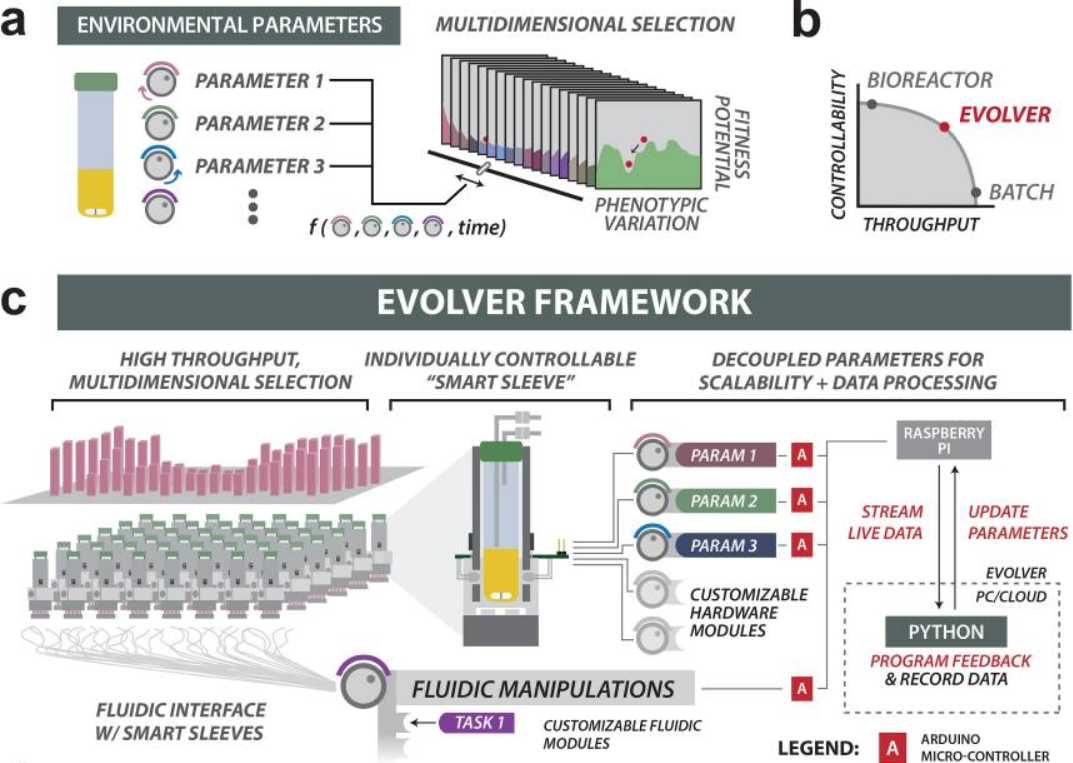
\includegraphics[width=1\columnwidth]{figures/intro_evolver.png}
\caption[Integrated framework of eVOLVER for high-throughput ALE experiments]{Integrated framework of eVOLVER for high-throughput ALE experiments.}
\label{fig:intro_evolver}
\end{center}
\end{figure}


Another simulator, ALEsim\cite{lacroix2017model}, was developed for the optimization of ALE experiments and promises to improve ALE results. It is a model built on the basic principles of growth in order to predict growth rates in batch cultures of ALE experiments (Figure \ref{fig:intro_alesim}). By evaluating various passage sizes, ALEsim can calculate how and when to deploy resources to shorten experiment timelines and to achieve desired results. ALEsim provides a way to design better experiments and quantify them, to obtain the desired outcome with the resources available on hand.

For a simulation using a developed model, experimental (i.e., culture size, passage size, passage optical density), statistical (i.e., number of experiments), and biological (i.e., beneficial mutation rate) parameters must be set for results to be biologically meaningful. These parameters can differ for different strains and conditions, and it is crucial to define the parameters for models to be constrained. ALEsim provides an advantage by allowing automated simulations, with the cells being allowed to grow under the user-defined conditions so that the experimental and biological parameters can be strictly controlled over the course of an experiment.

\begin{figure}[H]
\begin{center}
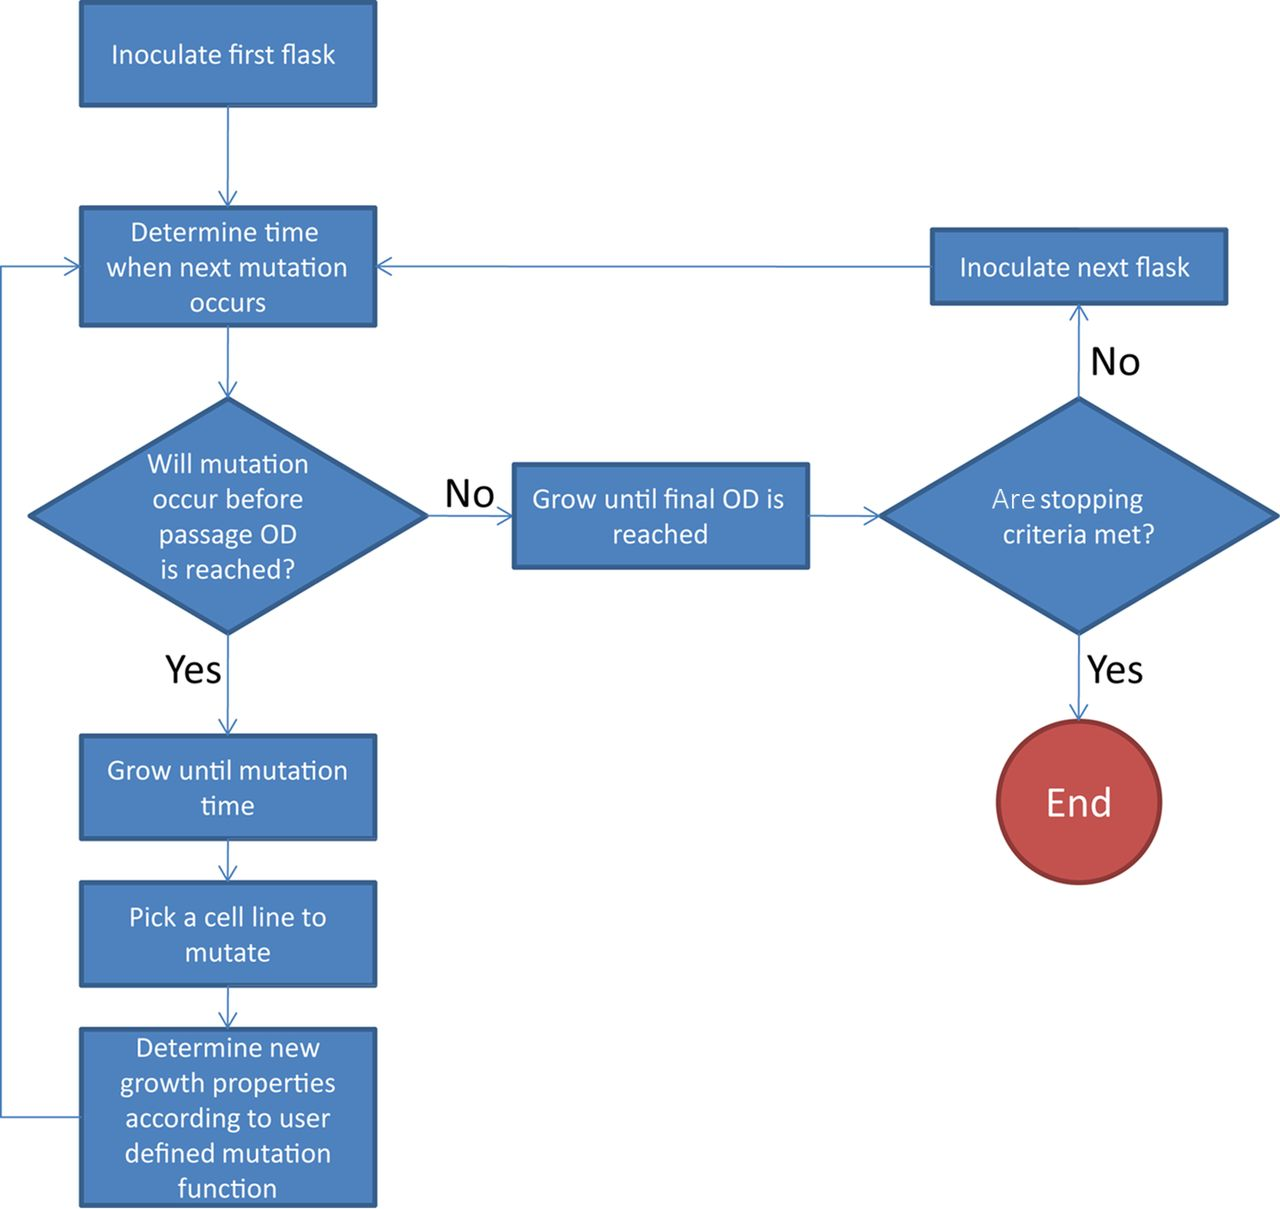
\includegraphics[width=1\columnwidth]{figures/intro_alesim.jpg}
\caption[ALEsim flow chart]{ALEsim flow chart.}
\label{fig:intro_alesim}
\end{center}
\end{figure}


\section{Systems Biology}
With the increasing availability of the computational tools and the development of high throughput techniques in the omics field, systems biology has shown a strong emergence in the last few years as a key multi-disciplinary field for integrating the multi-layer complexity of biological systems, particularly in the areas of transcriptomics, proteomics, metabolomics and fluxomics \cite{kitano2002systems}. This amount of available data allows researchers to investigate molecular cell processes in a large scales, applying theoretical, experimental and computational methods.

Biological systems based on complex interactions between various molecular components. The relations between these components are often obey nonlinear kinetics, for example, most of the reactions are regulated by one or more feedback or feed-forward loops with incomprehensible behaviors. When considered, cell structure and compartmentalization are also often introduce complexities to the unexpected behavior of the entire biological system \cite{bellouquid2006mathematical}. Mathematical modeling with these factors taken into consideration is used as a general approach to encompass existing knowledge in biological systems, and to gather information by analyzing these models to acquire a better understanding \cite{kremling2013systems}.

A mathematical model of a cell can be approached by two different approaches in either a bottom-up or top-down directionality (Figure \ref{fig:systemsbiology}) \cite{bruggeman2007nature, shahzad2012application}. Top-down approach is an experimental oriented approach, it starts from the whole picture and aims to characterize biological mechanisms closer to the smaller parts and their interactions in the network. In the bottom-up approach, collected data from biological knowledge is used as a starting point, a subsystem is generated to deduce the functional properties of smaller points in the network. Combination of the pathway level models (bottom-up) into a model for the entire system level (top-down) is the ultimate goal in the systems biology therefore these approaches are complementary.

\begin{figure}[ht]
\begin{center}
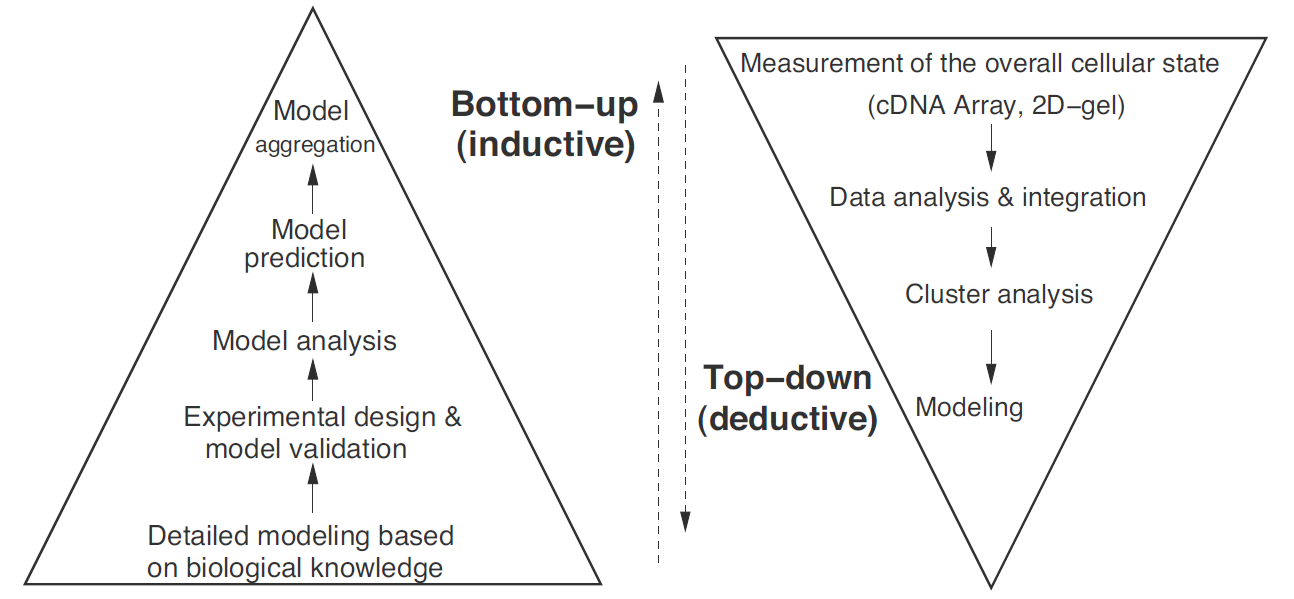
\includegraphics[width=0.8\columnwidth]{systemsbiology.png}
\end{center}
\caption[Systems biology approaches]{Systems biology approaches. Left: Bottom-up approach. Right: Top-down approach. Figure is taken from \cite{kremling2013systems}.}
\vskip\baselineskip % Leave a vertical skip below the figure
\label{fig:systemsbiology}
\end{figure}

\subsection{Metabolic Networks}   \label{metabolicnetworks}
In the context of systems biology, metabolic network reconstructions have become a common interest for the researchers over the past 20 years \cite{thiele2010protocol}. Organism-specific metabolic network analyses allow scientists to design experiments and even obtain beforehand predictions. These networks are the main sources of the mathematical models which can simulate metabolic fluxes reflecting the experimental reality \cite{orth2010flux}.

Before the improvement of genome sequencing or annotation technologies, initial core metabolic networks were based on the accessible information of biochemical pathways \cite{vallino1994carbon} \cite{varma1993biochemical}. In the last decade, larger genome-scale metabolic models (GSMMs) have been able to be developed rapidly with the help of databases for annotated genomes, providing information on substrates and products of each enzyme and each bioreaction \cite{feist2009reconstruction}. Growing biochemical databases provide automatization processes for the metabolic network reconstructions. As a result, genome-scale metabolic networks are available today for almost all organisms with an annotated genome available in the literature \cite{pitkanen2014comparative, kerkhoven2014applications}. From the first genome-scale metabolic model of \emph{Escherichia coli} to other organisms, the steps are required for GSMM development remained the same regardless of the biological diversity.

A generally applicable protocol is defined by the Palsson group \cite{thiele2010protocol, feist2009reconstruction} for the reconstruction of biochemical networks described in the Figure \ref{fig:modelreconstruction} \cite{chen2012metabolic}. Briefly, genomic data for the biochemical reactions of an organism are identified from the databases, such as NCBI, DDBJ and EMBL-EBI. Extraction and processing of the gene-protein-reaction relationship (GPR) of the genomic data results a draft reconstruction. GPR associations in the draft model should be reviewed by the researchers and manually curated if the identifying process is achieved with the help of automated computational algorithms \cite{pitkanen2014comparative}. Since the genomic data is the least representative of the biological phenotypes, available transcriptomic, proteomic, metabolomic and/or subcellular localization data are also used to further curate the model. Once the final metabolic network is reconstructed with bibliographic information, it is translated into a mathematical model.

\begin{figure}[ht]
\begin{center}
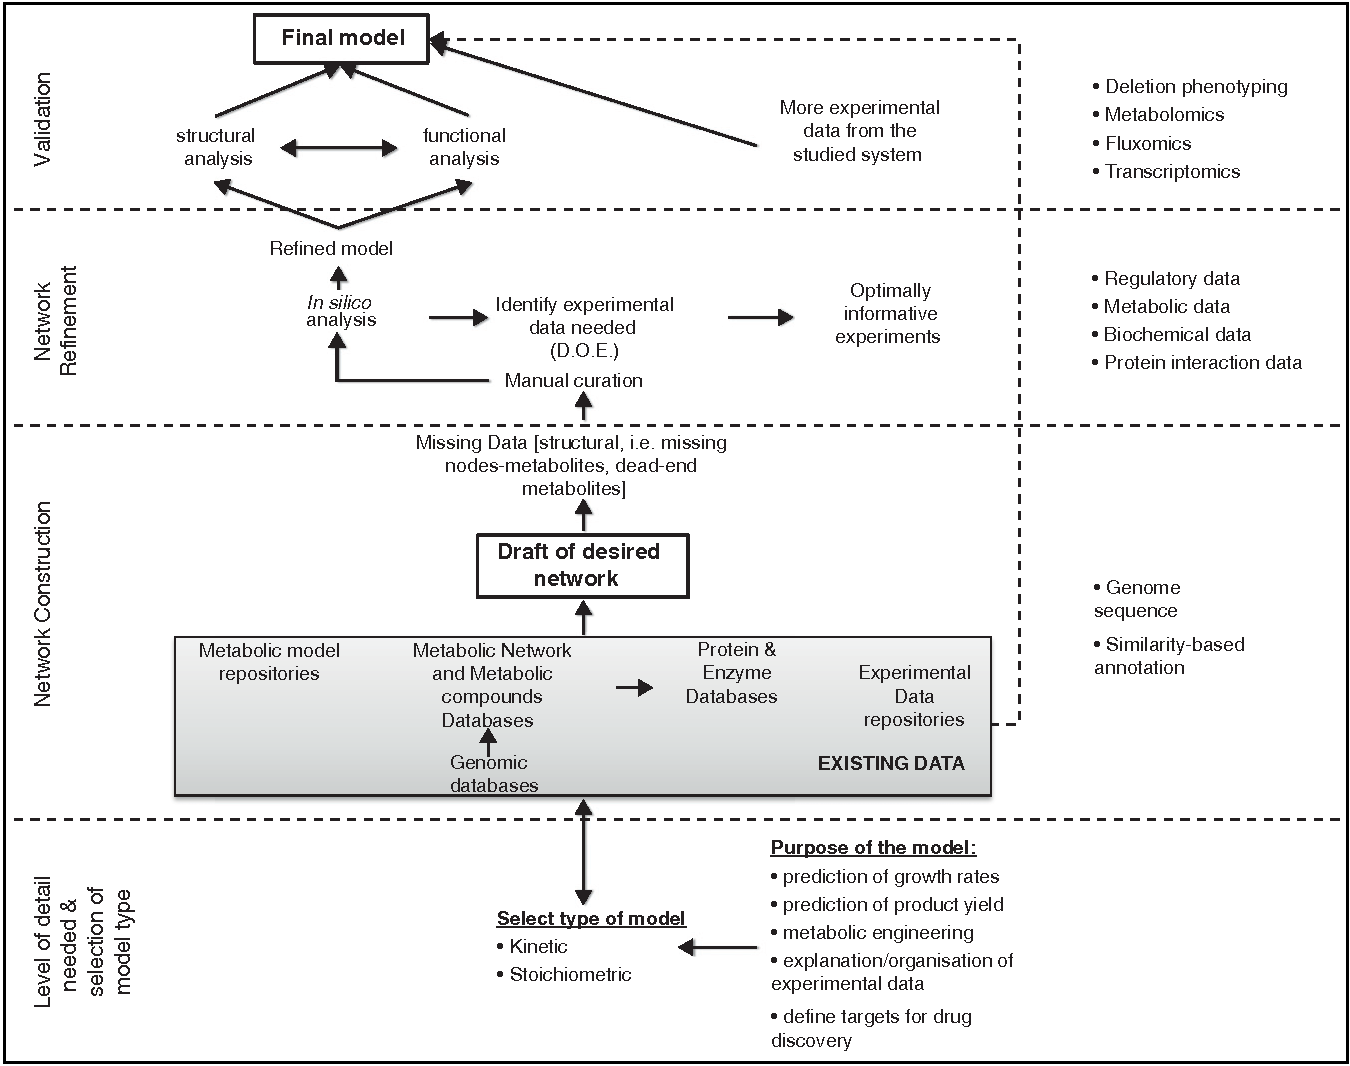
\includegraphics[width=1\columnwidth]{modelreconstruction.png}
\end{center}
\caption[Overview of metabolic network reconstruction protocol]{Overview of metabolic network reconstruction protocol. Figure is taken from \cite{chen2012metabolic}.}
\vskip\baselineskip % Leave a vertical skip below the figure
\label{fig:modelreconstruction}
\end{figure}

Once a metabolic network is reconstructed, a rational link between a genome sequence, the proteins encoded in the genome, and the reactions catalyzed by the proteins allowing to investigate the relationships between genotype and phenotype is achieved \cite{durot2008genome}. As the final step, GSMM needs to be validated by the new experimental data sets. GSMM validation process for various experimental conditions require detailed cultivation data from experiments. For example, information on the biomass composition of the specific organism leads more accurate biomass equation in the model, that is one of the key factors in the GSMM optimization and validation \cite{dikicioglu2015biomass}. Even tough multiple steps in the GSMM reconstruction can be achieved with the automated softwares available, it is usually necessary to curate the obtained model manually.

Approaches for analyzing metabolic networks are mainly categorized as dynamic or structural approaches. Even though the former is promising more realistic approach, its implementation in the literature is obstructed due to the unavailability of kinetic parameters for the majority of enzymes within a metabolic network \cite{machado2014systematic, ramkrishna2012dynamic} Because of the lack of kinetic parameters, structural metabolic modeling has been widely used for analyzing cellular metabolism at a steady-state assumption as a kind of snapshots taken at specific times.

GSMMs are one of the most useful tools in systems biology, especially in metabolic engineering studies \cite{kim2012recent}. In 1998, with the publication of \emph{Metabolic Engineering: Principles and Methodologies}, the term metabolic engineering is defined as the optimization of natural processes within cells to increase the production of certain substances \cite{stephanopoulos1999metabolic}. Hence, studies of metabolic engineering can be considered as genetic engineering in strain development. However, while metabolic engineering manipulates strains by altering flux distributions in the pathways; genetic engineering modifies specific genes, proteins and/or enzymes of interest \cite{stephanopoulos2012synthetic}. Although GSMMs are mainly used in metabolic engineering strategies, other applications both for descriptive and predictive purposes can be found in the literature \cite{osterlund2012fifteen}.

The ultimate goal of the GSMM reconstruction is to predict flux distribution profiles as close \emph{in silico} as they are \emph{in vivo}. Hence, GSMMs are in continuous research to improve predictability of organism-specific models.

\begin{figure}[ht]
\begin{center}
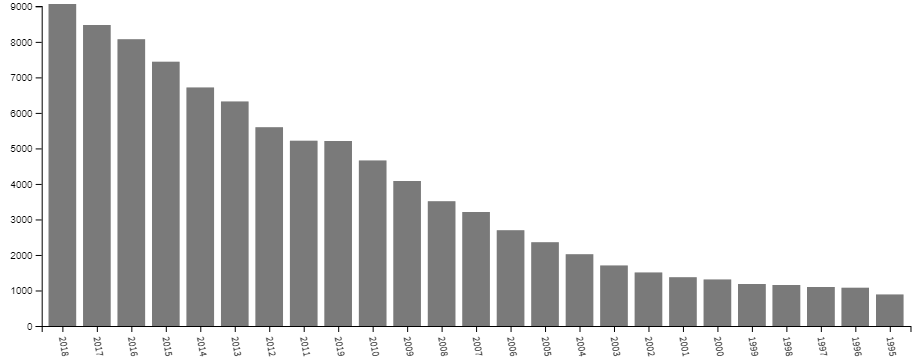
\includegraphics[width=1\columnwidth]{figures/intro_wos.png}
\end{center}
\caption[Web of Science article counts on the query "metabolic model" keyword]{Web of Science article counts on the query "metabolic model" keyword.}
\label{fig:wos_metabolicmodel}
\end{figure}

\subsection{Mathematical Representation of Metabolic Networks}
Basic applications of metabolic network modelling, although its framework is developed by engineers or mathematicians, is used by biologists with various mathematical backgrounds \cite{pinzon2018mathematical}. In order to speak with one voice, fundamental concepts of mathematical representation of metabolic networks in GSMM reconstructions will be provided in this section.

One can propose a steady-state model for the correlation between the metabolites exist in the network. This model claims that the production and consumption of a metabolites must balance each other \cite{reimers2016steady}. For example, consider the metabolite "A" in the toy network in Figure \ref{fig:ToyNetwork}. It can be taken into cell with the rate of b1, and can be converted into B or C with the rates of v1 and v2 respectively; at the same time, metabolite C can be converted into A with the rate of v3. Note that enzyme kinetics are not considered, and these equations are formed only considering mass balances.

\begin{figure}[h]
\begin{center}
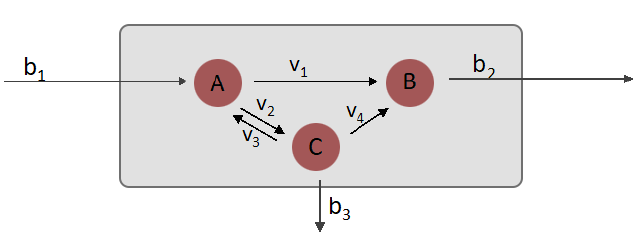
\includegraphics[width=1\columnwidth]{figures/intro_toymodel.png}
\end{center}
\caption[Toy network for steady-state assumption]{Toy network for steady-state assumption.}
\label{fig:ToyNetwork}
\end{figure}

If we accept the steady-state assumption, and since we know all the possible reactions passing through metabolite A, we can write following differential equation

\begin{equation}
 \ \frac{d(A)}{dt} = - v_1 - v_2 + v_3 + b_1 = 0 \\
\end{equation}


meaning that production rate of metabolite A is equal to its consumption rate. In other words, there will be no accumulation of metabolite A in the cell. Considering we have 3 metabolites and 7 reactions; this representation of reactions can be written as a system of linear equations:
\begin{figure}[h]
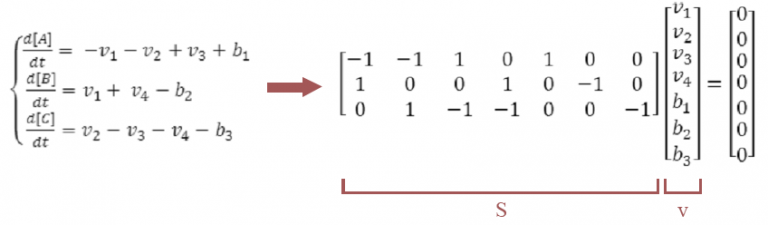
\includegraphics[width=1\columnwidth]{figures/intro_toymodel_eq.png}
\begin{center}S . v = 0 \end{center}
\end{figure}

In the above equation, a matrix "S" appears. S matrix consists of stoichiometric coefficients of the reactions. A single column of S matrix, representing a single reaction, provides information about the connections between the metabolites participating in that reaction; and a single row of S matrix, representing a metabolite, provides information about the connection of all the reactions in which that metabolite participates.

Next to S matrix a vector "v" appears. Vector "v" is called the flux vector, and it contains the change in concentration of metabolites. In other words, flux vector represents the flow rates or "fluxes" of each metabolite over time.

The solution space of S matrix, in the steady-state assumption, is generated by the null space base vectors of S. Studying on the null space vectors, we can define dead-end reactions (zero rows which mean reactions cannot carry flux), enzyme subsets (rows of scalar multiplies of each other, possibly chain reactions) and independent components (diagonal block structures in the null space, reactions that are independed from the network). Due to the large number of reactions in biological networks, the system is underdetermined and have multiple solutions in a convex flux cone space, referring to multiple steady-states of the cell.

\subsection{Constraint-Based Modelling}
As explained in the previous section, solution of a metabolic network is not unique, meaning that the model can be found in multiple states of flux distributions. In order to obtain more biologically relevant solutions, v vector can be calculated within a set of constraints \cite{thiele2007bringing}. The rationale behind constraining the flux vector is that biological systems must obey general principles in nature, such as basic rules of chemistry and the laws of thermodynamics.

In terms of physico-chemical properties of a biological system, mass and charge balance must be conserved. These conservation laws are given into mathematical problem as "hard" constraints since these rules are inviolable \cite{price2004genome}. Reaction reversibility is a hard constraint, determined by the laws of thermodynamics. Some reactions are irreversible by nature under certain conditions. These reactions are mathematically bounded in the flux vector, so they can have only positive (vi ≥ 0, forward directionality) or negative (vi ≤ 0, backwards directionality) values. Depending on the methodology, by reversing the equations of backwards-directed reactions, and splitting the reversible reactions into two forward and reverse reactions, one can obtain a vector v where each element is greater than or equal to 0.

Since the experiments are carried out in a defined medium, environmental constraints must be added in silico simulations as well. These constraints include nutrient availability (such as carbon, nitrogen, or oxygen sources), the pH value, temperature, or any other experiment-specific conditions. Additionally, spatial constraints can be given to the system to limit substrate and enzyme availability for a specific compartment, especially for the metabolites which are transferred between compartments by facilitated diffusion.


There are several methods used in constraint-based modelling (Figure \ref{fig:intro_constraintbasedmodelling}) and additional constraints are introduced into the field every day. More recently, regulatory constraints have started to be used to simulate experimental observations on cellular regulatory mechanisms, such as variable amounts of gene products (transcriptional, translational regulations) and their activities (enzymatic regulations). Integration of omics data, mainly transcriptome data, is used to capture these regulations in silico.


\begin{figure}[H]
\begin{center}
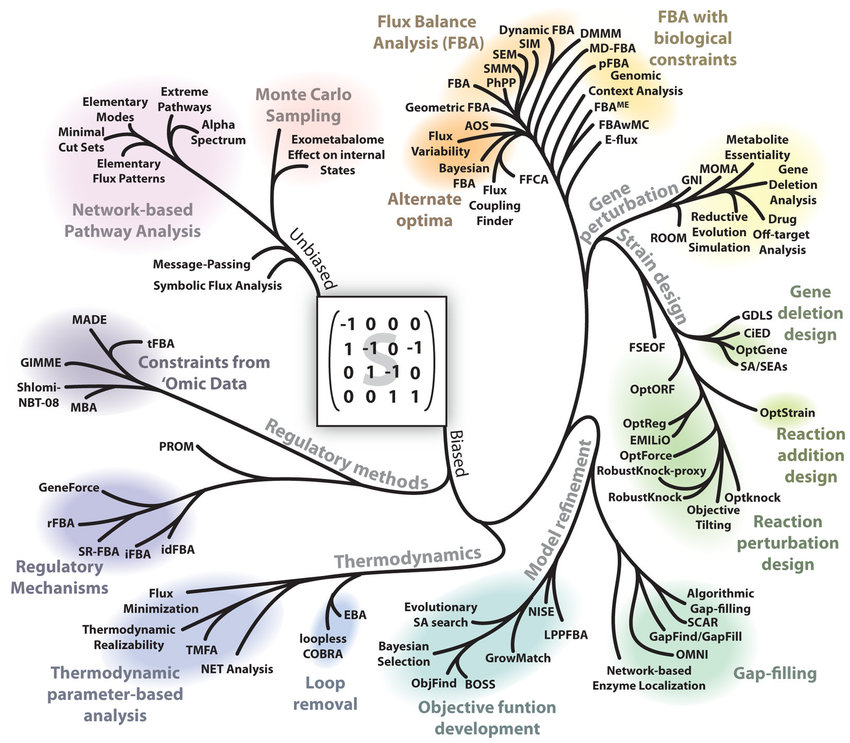
\includegraphics[width=1\columnwidth]{figures/intro_constraintbasedmodelling.png}
\end{center}
\caption[Various constraint-based modeling methods]{Various constraint-based modeling methods \cite{lewis2012constraining}.}
\label{fig:intro_constraintbasedmodelling}
\end{figure}



\section{\emph{Saccharomyces cerevisiae}}

The species "yeast" includes a range of eukaryotic single-celled microorganisms, although it is commonly used to describe \emph{Saccharomyces cerevisiae}. Also known as the baker's yeast, \emph{S. cerevisiae} is one of the extensively used microorganisms for alcoholic fermentation of beverages, bio-ethanol production, and processing various foods since ancient times \cite{gelinas2009inventions}. It was the first eukaryotic organism whose genome was fully sequenced and annotated \cite{goffeau1997multidrug}, and besides its benefits in the industry, it is used as a model system for other eukaryotic cells including humans \cite{dujon1996yeast, botstein1997yeast}.

\subsection{Central Carbon Metabolism of \emph{S. cerevisiae}}
From the end of the eighteenth century, mainly after the fermentation is defined as "respiration without oxygen", the metabolism of \emph{S. cerevisiae} has been studied extensively \cite{barnett1998history, barnett2000history}. Its capability to produce ethanol is one of the most characterized microbial processes due to industrial utilization.

The set of anabolic and catabolic reactions in the cell are referred as the metabolism. A schematic representation of the central carbon metabolism in \emph{S. cerevisiae} can be found in Figure \ref{fig:central_carbon_mech_of_s_cerevisiae_kegg}. Glycolysis, pentose-phosphate pathway (PPP), tricarboxylic acid cycle (TCA) or Krebs cycle, the glyoxylate cycle and the electron transport chain are the main pathways in central carbon metabolism.

Glycolysis is a cytosolic pathway where 1 molecule of glucose breaks down into 2 molecules of pyruvates while 1 molecules of ATP on the substrate level and 2 molecules of NADH. Within the glycolysis, important precursors for biomass such as 3-phosphoglycerate, 3PG, PEP are generated. The final product of glycolysis, pyruvate, is an important branch point metabolite in the central carbon metabolism.

 \begin{figure}[H]
 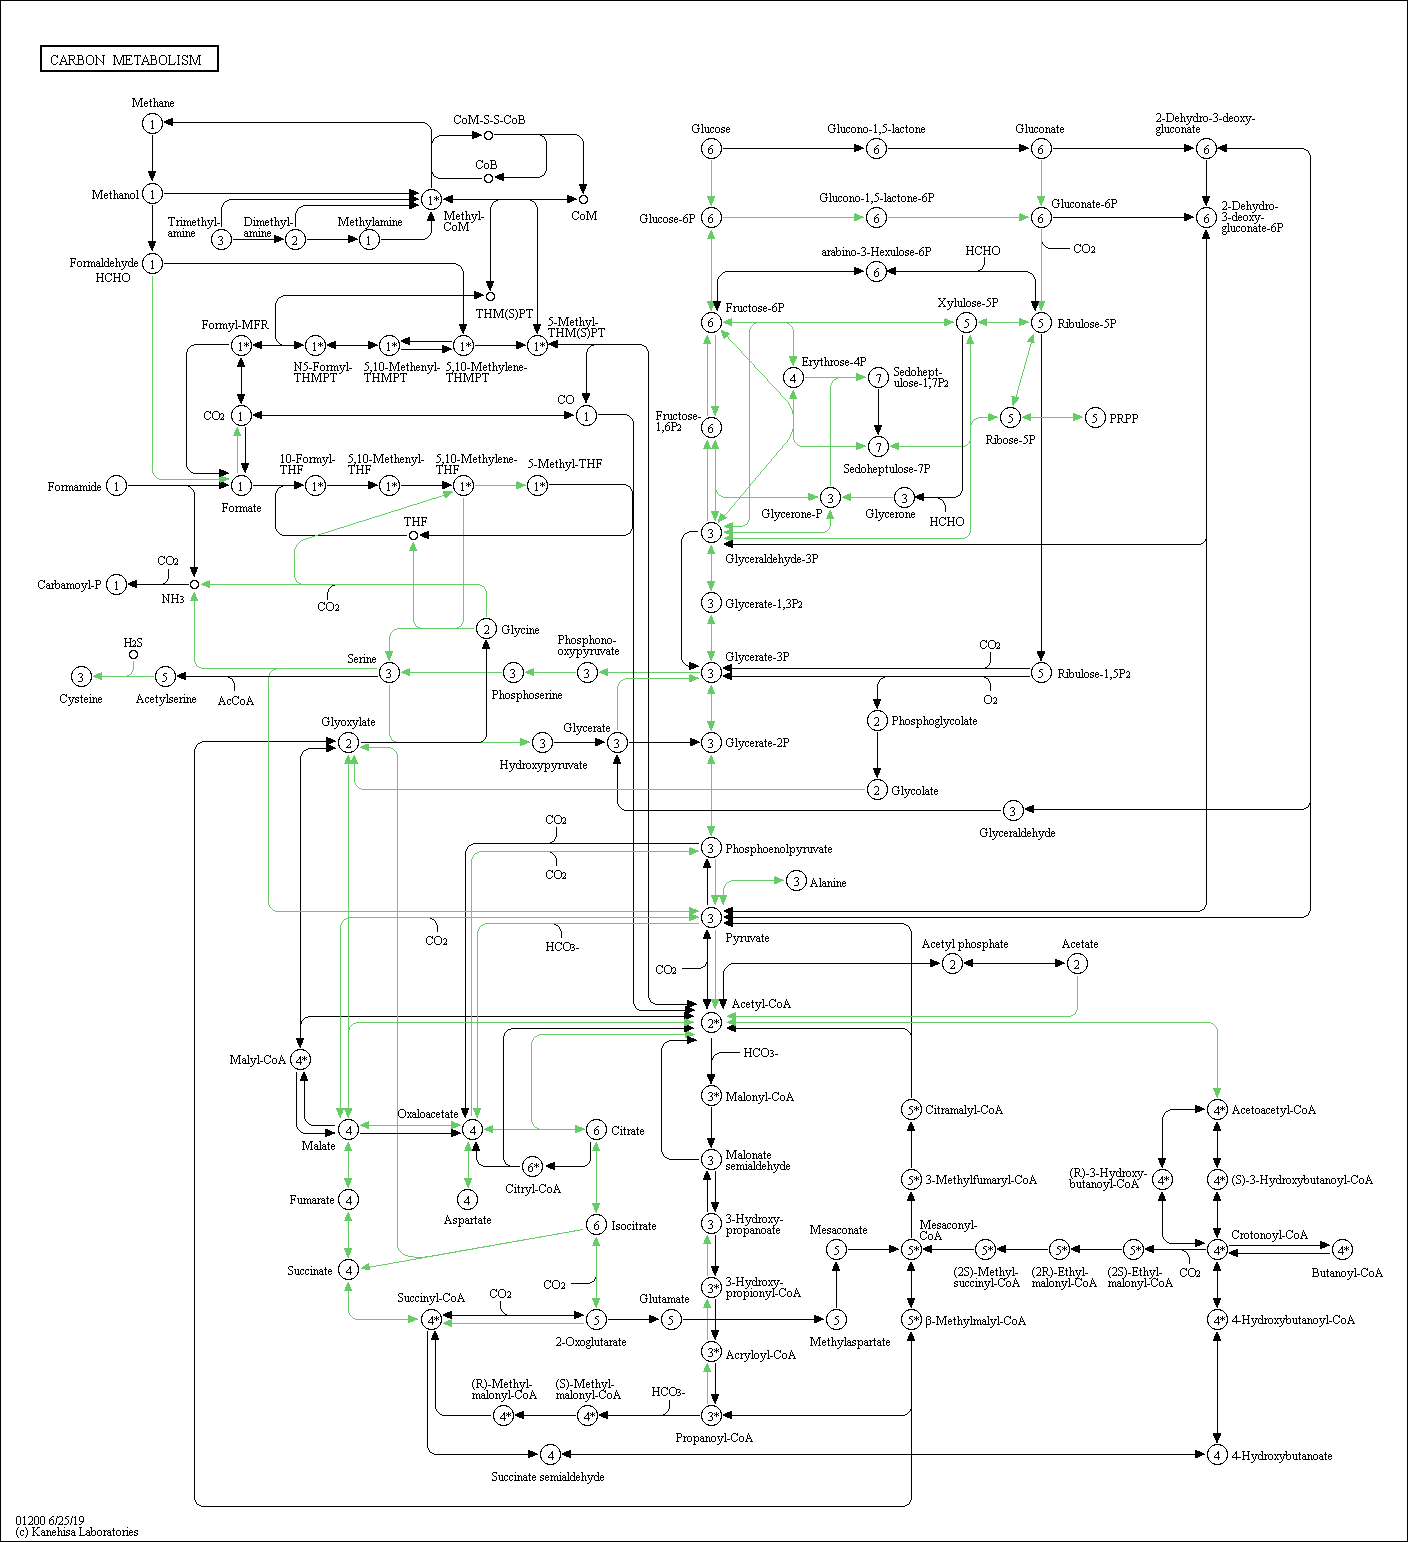
\includegraphics[width=1\columnwidth]{central_carbon_mech_of_s_cerevisiae_kegg.png}
 \caption[Central carbon mechanism of \emph{S. cerevisiae}]{Central carbon mechanism of \emph{S. cerevisiae} obtained from  KEGG \cite{kanehisa2000kegg}.}
 \vskip\baselineskip % Leave a vertical skip below the figure
 \label{fig:central_carbon_mech_of_s_cerevisiae_kegg}
 \end{figure}

The end product of glycolysis, pyruvate, can be converted into acetaldehyde through pyruvate decarboxylase (PDC) and, to ethanol with consumption of 1 NADH molecule by alcohol dehydrogenase (ADH). Acetaldehyde is also an important branch point metabolite and it can be converted into acetate by the acetaldehyde dehydrogenase (AcDH) with reduction of 1 NADP+ to NADPH. Acetate can be converted into acetyl-CoA by the acetate synthase (ACS) in the cytoplasm, and used as precursor for biosynthesis of secondary metabolites and in lysine biosynthesis. The stoichiometric reaction for the glycolysis can be found in Equation \ref{eq:glycolysis}.

\begin{align}
\begin{split}
\label{eq:glycolysis}
\ Glucose + 2 ADP + 2 P + 2 NAD^+ \xrightarrow{} \\
\ 2 Pyruvate + 2 ATP + 2 NADH + 2 H$_2$O + 2H^+
\end{split}
\end{align}

Some enzymes in the glycolytic pathway are regulated allosterically. For example, presence of ATP in the cytoplasm inhibits the hexokinase (HXK) which deactivates the first step of glycolysis \cite{larsson2000importance}. It is also known that during low concentrations of glucose-6-phosphate (G6P) and fructose 6-phosphate (F6P), mitochondrial oxidative phosphorylation enzymes are activated and it is antagonized by the fructose 1,6- bisphosphate (F1-6bP) \cite{diaz2008mitochondrial}. This phenomenon shows that the metabolite F1-6bP inhibits the respiratory flux rates.

To determine whether the regulation of metabolism was taking place at transcriptional and translational level or through metabolic regulation, microarray studies and obtained transcriptomic data are analyzed by ter Kuile and Westerhoff\cite{ter2001transcriptome}. By using mathematical modeling, they concluded that regulation is almost never completely at translational level and metabolic regulation points must be investigated. Daran-Lapujade, et al., found the correlation between transcript levels, flux profiles and enzyme activity is very little \emph{in vivo} \cite{daran2004role}.

Gluconeogenesis, as a form of a reversed glycolysis, generates glucose-6-phosphate (G6P) from amino acids (except lysine and leucine) and, C2 and C3 compounds. C2 compounds can also be converted into C4 dicarboxylic acids bypassing oxidative decarboxylation through glyoxylate cycle. During fully respiratory conditions, if the available glucose ratio is above 1\%, synthesis of the enzymes for glyoxylate cycle is repressed while oxidative decarboxylation is bypassed. Although this pathway is considered as a modification of the TCA cycle, the localization of this pathway is still unknown.

\begin{figure}[H]
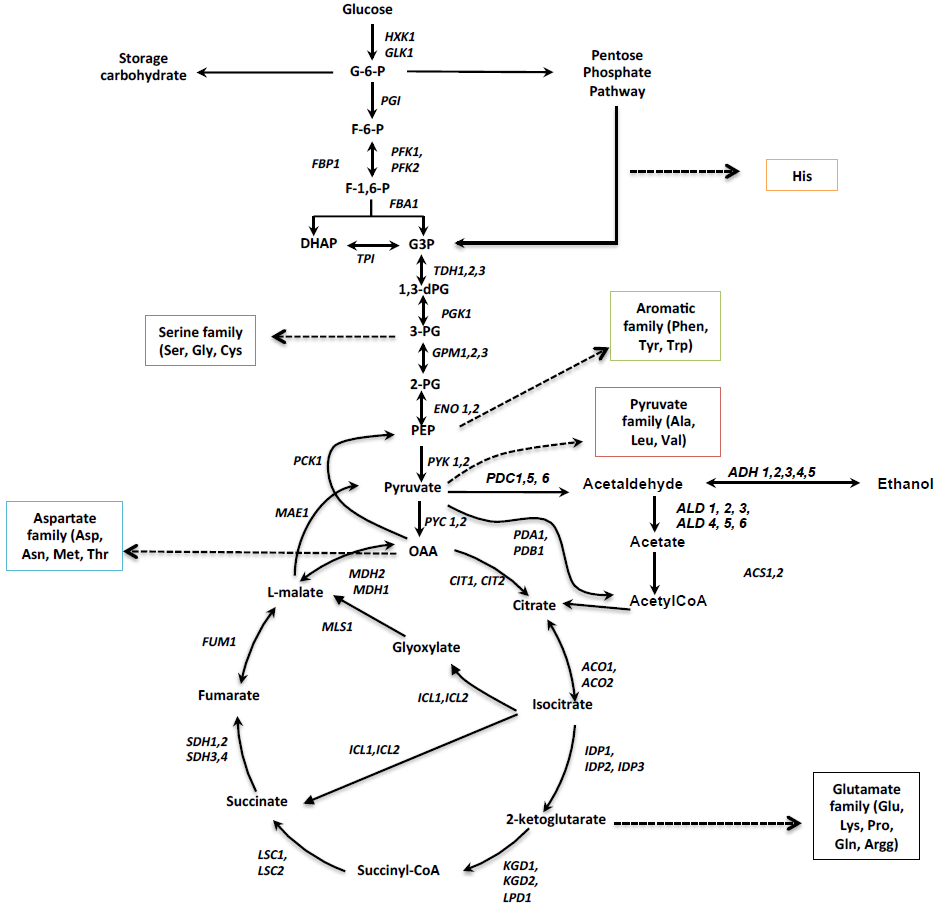
\includegraphics[width=1\columnwidth]{figures/intro_centralcarbon.png}
\caption[Diagram of pathways (glycolytic pathways, pentose phosphate pathway, TCA cycle, glyoxylate cycle) involved in the central carbon metabolism of \emph{S. cerevisiae}]{Diagram of pathways (glycolytic pathways, pentose phosphate pathway, TCA cycle, glyoxylate cycle) involved in the central carbon metabolism of \emph{S. cerevisiae}.}
\label{fig:intro_centralcarbon}
\end{figure}

Krebs cycle or the citric acid cycle (TCA cycle for short), forms the compounds NADH, CO$_2$ and FADH2. For 1 mole of pyruvate oxidized in TCA cycle, 4 mol of NADH, 1 mol of FADH2, 3 mol of CO$_2$ and 1 mol of GTP are generated. The overall stoichiometric reaction for the TCA cycle can be found in Equation \ref{eq:TCA}.

\begin{align}
\begin{split}
\label{eq:TCA}
\ Pyruvate + 3 H$_2$O + GDP + 2 P + 4 NAD^+ + FAD \xrightarrow{} \\
\ 3 CO$_2$ + GTP + 4 NADH + FADH$_2$ + 4 H^+
\end{split}
\end{align}

The TCA cycle is mostly regulated at transcriptional level and it is known that the cycle is repressed by high glucose concentrations \cite{liu1999transcriptional}. The main regulatory points in the TCA cycle are the citrate synthase, isocitrate dehydrogenase and α-ketoglutarate dehydrogenase. The cycle is also regulated by feedback inhibition mechanisms and regulation is highly controlled at enzymatic level. For example, the isocitrate dehydrogenase (IDH) is increases its activity with the presence of AMP and inhibited by the presence of ATP\cite{coleman1975regulation}; while the low level of NADH/NAD+ molecules activates the majority of enzymes in the cycle \cite{gadde1997mutations}. The TCA cycle is a major pathway in mitochondria and it is used to generate important precursor metabolites such as citrate, oxaloacetate, and succinyl-coA.

The reduced cofactors generated from metabolic pathways in the mitochondrial matrix, such as NADH molecules, are re-oxidized to H$_2$O molecules by NADH:ubiquinone oxidoreductase (also called internal NADH dehydrogenase) which is localized on the inner membrane on mitochondria \cite{bakker2001stoichiometry}. This oxidation process is called mitochondrial respiration, or oxidative phosphorylation, and it provides a way to the cell to generate energy in the form of ATP molecules. NADH molecules generated in the cytosol can also be oxidized in yeast by external NADH dehydrogenase, or it can be taken inside mitochondria via glycerol-3-phosphate shuttle to be coupled with the respiratory chain, where the ubiquinone pool donates \cite{zitomer1979transcriptional} its electrons to the cytochrome-c through the bc1-complex, and oxidation of cytochrome-c by is catalyzed by cytochrome-c oxidase \cite{de1987mitochondrial}. Similar to NADH molecules, produced FADH2 molecules in the TCA cycle (during oxidation of succinate into fumarate) act as electron donors for ubiquinase \cite{cimini2009global}.

Overall, the central carbon metabolism is finely tuned throughout the organic evolution to supply required energy and to produce building blocks for a yeast cell. All the pathways mentioned are interconnected through metabolites (reaction products or substrates) and/or cofactors (such as ATP, NAD, and NADP) within the cell. These pathways are activated or down-regulated by a tight regulation in order to satisfy what is required according to environmental conditions.

The most characterized regulatory effects of yeasts can be listed as 1) Pasteur Effect, the inhibition of fermentation in the presence of oxygen with a decreased affinity for sugar uptake \cite{lagunas1983role}, 2) Kluyver Effect, for the species \emph{Candida utilis}, \emph{Kluyveromyces wickerhamii} and \emph{Debaryomyces yamadae}, being able to ferment glucose anaerobically but not being able to ferment maltose, lactose, and sucrose \cite{kaliterna1995transient}, 3) Custer Effect, the species \emph{Dekkera} and \emph{Brettanomyces} ferment glucose to ethanol faster under aerobic conditions \cite{scheffers1966stimulation}, and 4) Crabtree Effect, the suppression of respiration by high glucose condition.



\subsection{Adaptive Evolution Studies on \emph{S. cerevisiae}}

Various strategies for evolutionary engineering in \emph{S. cerevisiae} are developed throughout the years. These strategies can be collected as 1) serial transfers in shake flasks, 2) sequential batch reactor cultivations, 3) continuous cultivations, 4) dynamic selection regimes, and 5) synthetic selection circuits \cite{mans2018under}.

Ho, Ping-Wei, et al. successfully obtained a faster glycerol utilization in two evolved derivatives of the strain CEN.PK113-1A by serial transfer in synthetic medium with glycerol as sole carbon source. After 55 generations, evolved strains were able to grow in synthetic glycerol medium, and evolved strains showed a higher growth rate on glycerol \cite{ho2017sole}.

New \emph{S. cerevisiae} strains that grew as fast in the absence of biotin as in its presence are obtained by Bracher, Jasmine M., et al \cite{bracher2017laboratory}. The evolved strains were obtained by sequential batch reactor cultivation on synthetic medium in the absence of biotin, and showed 32-fold increased maximum specific growth rates.

Smith, Van Rensburg, and Görgens improved xylose fermentation in \emph{S. cerevisiae} strain D5A+ in the presence of lignocellulosic inhibitors by ethyl methanesulfonate (EMS) mutagenesis and anaerobic chemostat cultivation after 100 generations\cite{smith2014simultaneously}. The study showed that the laboratory evolution profoundly altered the yeast metabolism, provided that evolved strains achieved 7.5-fold reduction of lag phase and were able to remove HMF, furfural and acetic acid completely in 24 h.

Ethanol tolerance is the most important trait of industrial yeasts, and the ability to grow in high levels of ethanol is an industrially desired feature without question. Voordeckers, Karin, et al. improved ethanol tolerance
in S288c strain FY5 by aerobic turbidostat cultivation on complex medium with gradually increasing concentrations of ethanol (from 6\% up to 12\%). After 200 generations, up to 2.5-fold increased fitness achieved in medium containing 9\% ethanol and growth in the presence of 12\% ethanol \cite{voordeckers2015adaptation}.

\subsection{Metabolic Models of \emph{S. cerevisiae}}
After the first \emph{S. cerevisiae} genome sequence is published, the first cDNA spotted microarray exploring metabolic gene regulation in 1997 \cite{derisi1997exploring}, and the first commercial platform for oligonucleotide microarray data (Affymetrix) to investigate cellular regulations were reported in 1998 \cite{cho1998parallel}. Existing genome data is integrated with the extensive annotation based on microarray data and biochemical knowledge from literature, leading of the publication of the first GSMM of \emph{S. cerevisiae} in 2003 \cite{forster2003genome}.

The first genome-scale model of S. cerevisiae, iFF708, contained a total of 1175 reactions, 708 genes and 584 metabolites compartmentalized between the cytosol and mitochondrion. The model was validated and used in \emph{in-silico} gene deletion studies\cite{forster2003large} and the calculation of physiological parameters\cite{famili2003saccharomyces}.

From the first model reconstruction, more biologically accurate data were integrated into models such as the logical relationship between genes (GPR associations), the comprehensive conservation of mass and charge through elementally and charge-balanced reactions (proton balance), and the full compartmentalization of metabolites and proteins. iND750, the second genome-scale metabolic model of \emph{S. cerevisiae} contained 1149 unique reactions, 750	genes, 646 metabolites and five additional compartments (peroxisome, nucleus, golgi apparatus, endoplasmic reticulum, and vacuole)\cite{duarte2004reconstruction}.

\begin{figure}[H]
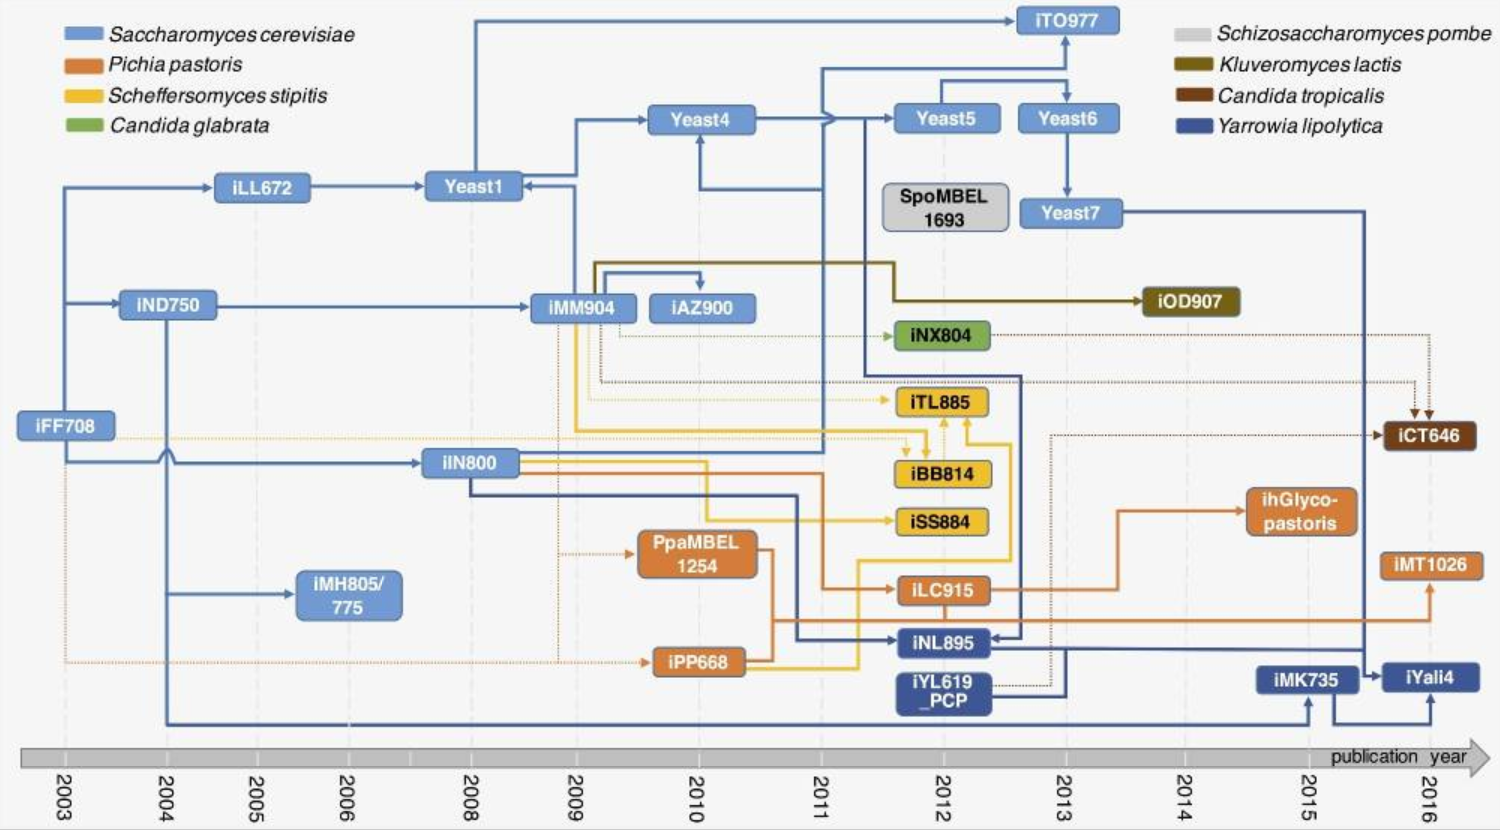
\includegraphics[width=1\columnwidth]{figures/intro_yeastgemschronology.png}
\caption[Evolutionary timeline of different yeast species genome-scale metabolic models]{Evolutionary timeline of different yeast species genome-scale metabolic models.}
\label{fig:intro_yeastgemschronology}
\end{figure}

Afterwards, the model iLL672 was reconstructed based on the older iFF708 with improved connectivity of the network\cite{kuepfer2005metabolic}. Previous models were reconciled by deleting duplicates and multiple dead-end reactions, resulting a model with a total of 636 metabolites and 1038 reactions. Improvements of the metabolic models are followed by the iIN800 \cite{nookaew2008genome}, which tRNA synthesis, transport processes and a detailed lipid metabolism included.

Later, an improved version of the iND750 model, named iMM904, is reconstructed introducing a new database-independent nomenclature for 1226 metabolites, 1577 reactions, and 905 genes such as SMILES or InChI strings \cite{mo2009connecting}. The idea behind the reconstruction of the iMM904 was to provide a common model that serves as a base for studying the systems biology of yeast. Additionally, authors claimed that the  integration of the exometabolomic data into the model allowed to essentiality predictions using GSMMs.

Corrections to the iMM904 model formed the next model, named iAZ900 containing 900 genes, 1240 metabolites and 1602 reactions distributed among seven compartments \cite{zomorrodi2010improving}. In addition to the corrections on reversibility of the reactions, GPR associations and biomass definition, revision of the previous model included addition/removal of reactions, metabolites and/or genes.

\begin{figure}[H]
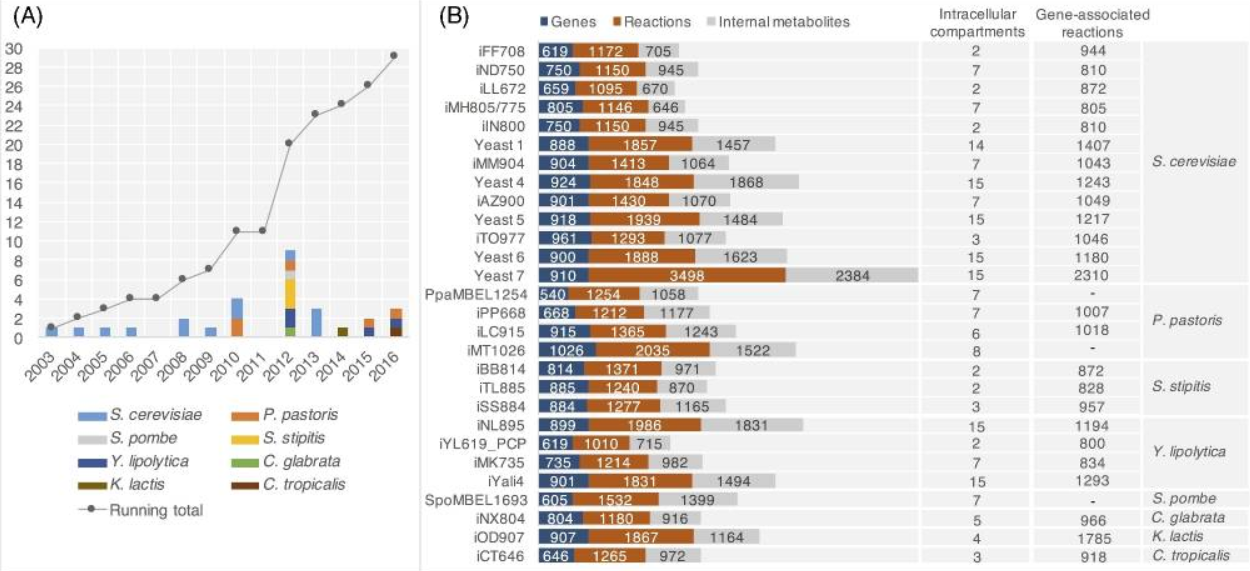
\includegraphics[width=1\columnwidth]{figures/intro_yeastgemschronology2.png}
\caption[Published genome-scale models of yeast in gene, reaction, metabolite and compartment numbers]{Published genome-scale models of yeast in gene, reaction, metabolite and compartment numbers.}
\label{fig:intro_yeastgemschronology2}
\end{figure}

Yeast1, the first collaboratively constructed consensus genome-scale metabolic network was built using standardized identifiers \cite{herrgaard2008consensus}. The consensus model was cumulatively improved despite its inability to perform computational simulations. With Yeast4 \cite{dobson2010further}, which includes metabolite transport reactions, an improved lipid metabolism (based on iIN800) and improved network connectivity, a consensus model was able perform simulations. Following updates on the consensus model included expansions on the lipid metabolism with Yeast 5 \cite{heavner2012yeast}; improved predictions with Yeast 6\cite{heavner2013version}; and major changes in the fatty acid, glycerolipid, and glycerophospholipid metabolisms with Yeast 7 \cite{aung2013revising} models. The latest version of the consensus model of \emph{S. cerevisiae}, Yeast8 \cite{lu2019consensus}, is released in the last year and continues to be updated by the community.


\subsection{Applications of \emph{S. cerevisiae} GSMMs}
Several genome-scale metabolic models of \emph{S. cerevisiae} have been used in metabolic engineering applications. These studies were mostly carried out for the development of yeast cell factories to increase yield industrially. Despite the high number of GSMM availability, only a selection of the models has been successfully validated experimentally.

For improved bioethanol production, Bro et al. simulated a number of strategies that increased ethanol yields under anaerobic conditions using the model 	iFF708\cite{bro2006silico}. FBA analyses showed the alterations on the redox metabolism, and the resulting strain had reduced glycerol yield 40\% on glucose and increased ethanol yield (+3\%) with the same maximum specific growth rate.

iMM904 model is successfully used with Optknock framework \cite{burgard2003optknock} (an FBA-based algorithm to predict gene deletion strategies) and new industrially preferable strains, which has improved 2,3-butanediol production, were designed. This successful implementation was the first report about increased 2,3-butanediol yield, and designed strains were validated experimentally \cite{ng2012production}.

Another report was the producing fumaric acid by direct fermentation in yeast, using the model iND750 \cite{xu2012fumaric}. This prediction was also based on literature mining, i.e. the target gene was selected after intense research, and FBA analyses on the metabolic model showed that deletion of the selected gene can lead to fumaric acid production without any significant change in growth rates.

The same iMM904 model was also used by Sun et al., to obtain a strain with 8- to 10-fold increased amorphadiene product yield compared to the wild type \cite{sun2014identification}. Results gathered by identifying the knockout positions with a potential to promote terpenoid production in the cell. Predictions were validated by the constructed single mutant and the study indicated that the metabolic models are powerful tools in the engineering of knockout strains before performing any molecular manipulations.
